%\subsection{UCW11 - Visualizza informazioni locale}
\begin{figure}[!h]
\centering
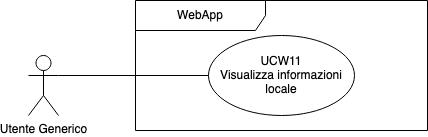
\includegraphics[scale=0.5]{UC_images/UCW11.png} 
\caption{UCW11 - Visualizza informazioni locale}
\end{figure}
\begin{itemize}
    \item \textbf{Descrizione}: L'utente generico visualizza le informazioni di un locale.
    \item \textbf{Attore primario}: Utente generico.
    \item \textbf{Precondizione}: L'utente ha svolto la funzione di ricerca di un locale o sta visualizzando la classifica dei locali.
    \item \textbf{Postcondizione}: Vengono visualizzate le informazioni di un locale:
    \begin{enumerate}
        \item Nome del locale;
        \item Descrizione del locale;
        \item Indirizzo del locale;
        \item Punteggio del locale;
        \item Numero di telefono del locale;
        \item Sito web del locale.
        \end{enumerate}
    \item \textbf{Scenario principale}: 
    \begin{enumerate}
    \item L'utente seleziona un locale tra quelli presenti nella lista;
    \item Il sistema mostrerà all'utente le informazioni relative al locale scelto.
    \end{enumerate}
\end{itemize}